\documentclass[11pt, a4paper]{article}
\usepackage[latin1]{inputenc}
\usepackage{pgfplots}
\usepackage{pgfplotstable}
\pgfplotsset{width=\textwidth ,compat=1.9}
\usepackage[dutch]{babel}
\usepackage{csquotes}
\usepackage{amsmath}
\usepackage{amsfonts}
\usepackage{amssymb}
\usepackage[backend=biber, style=numeric, citestyle=numeric-comp, sorting = none]{biblatex}
\author{Stef Tweepenninckx, r0677232}
\title{Practicum 1: Sorteeralgoritmes}


%define printtitle
\makeatletter
\def\printtitle{                 
    {\large \@title}} 
\makeatother

%define printauthor
\makeatletter                       
\def\printauthor{                  
    {\large \@author}}              
\makeatother

\begin{document}
\begin{titlepage}
\newcommand{\HRule}{\rule{\linewidth}{0.5mm}} 
\center 
\textsc{\LARGE Gegevensstructuren en algoritmen}\\[1.5cm] 
\HRule \\[0.4cm]

{\huge \bfseries \printtitle}\\[0.4cm] 
\HRule \\[0.4cm]

\Large \emph{Authors:}\\
 \textsc{\printauthor}\\[3cm]

{\large \textsc{\today}}\\[3cm] 

\vfill 
\end{titlepage}

\section*{Aantal vergelijkingen}
\subsubsection*{Selection sort}
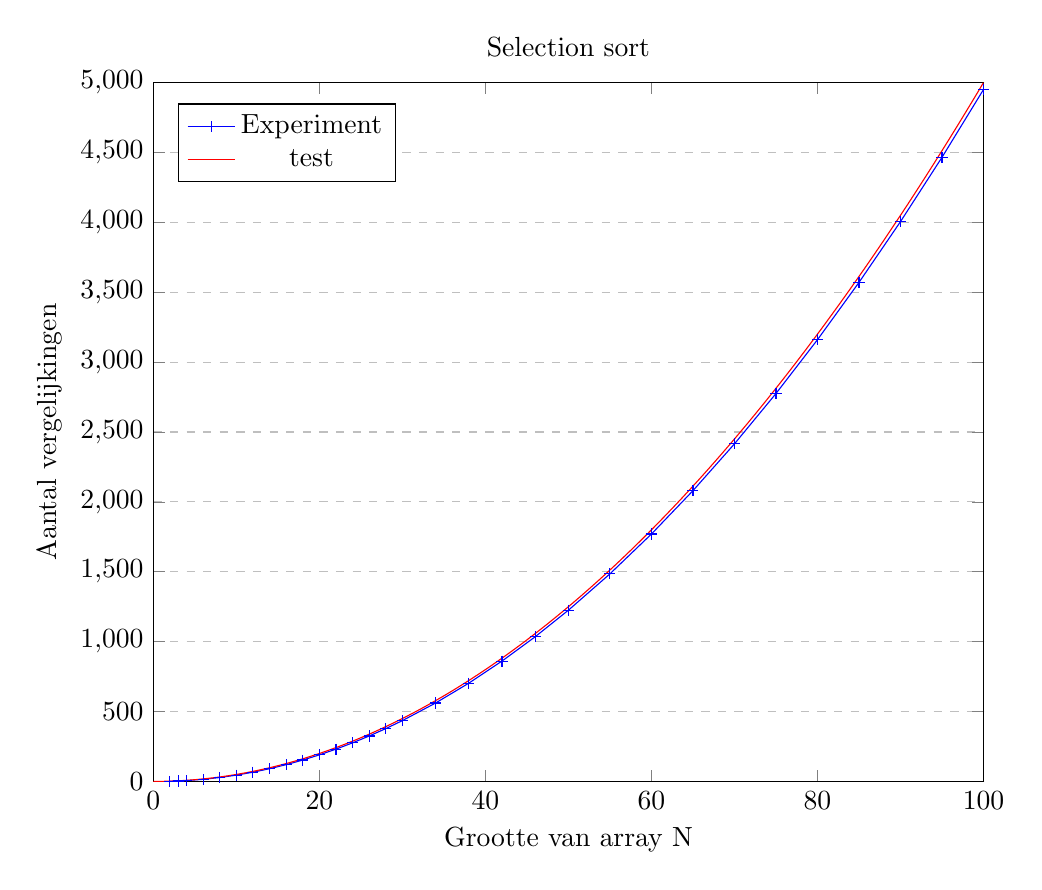
\begin{tikzpicture}
\begin{axis}[
    title={Selection sort},
    xlabel={Grootte van array N},
    ylabel={Aantal vergelijkingen},
    xmin=0, xmax=100,
    ymin=0, ymax=5000,
    xtick={0,20,40,60,80,100},
    ytick={0,500,1000,1500,2000,2500,3000,3500,4000,4500,5000},
    legend pos=north west,
    ymajorgrids=true,
    grid style=dashed,
]
 
\addplot[
    color=blue,
    mark=+,
    ]
    coordinates {
    (2,1)(3,3)(4,6)(6,15)(8,28)(10,45)(12,66)(14,91)(16,120)(18,153)(20,190)(22,231)(24,276)(26,325)(28,378)(30,435)(34,561)(38,703)(42,861)(46,1035)(50,1225)(55,1485)(60,1770)(65,2080)(70,2415)(75,2775)(80,3160)(85,3570)(90,4005)(95,4465)(100,4950)
    };
    \legend{Experiment};

\addplot [
    domain= 0:100, 
    samples=100, 
    color=red,
    ]
    {(x^2)/2};
    \addlegendentry{test};
	
 
\end{axis}
\end{tikzpicture}

\subsubsection*{Insertion sort}
\pgfplotstableread{
X Y
2 1
3 4
4 10
6 21
8 48
10 65
12 94
14 143
16 210
18 277	
20 312
22 373
24 452
26 587
28 626
30 771
34 1057
38 1367
42 1679
46 2043
50 2233
55 2687
60 3500
65 3598
70 4627
75 5399
80 6090
85 922
90 7775
95 8434
100 8924
}\datatable
\begin{tikzpicture}
\begin{axis}[legend pos=outer north east]
\addplot [only marks, mark = *] table {\datatable};
\addplot [thick, red] table[
    y={create col/linear regression={y=Y}}
] % compute a linear regression from the input table
{\datatable};
\addplot [
    domain= 0:100, 
    samples=100, 
    color=red,
    ]
    {(x^2)/4};

\addlegendentry{$y(x)$}
\addlegendentry{%
$\pgfmathprintnumber{\pgfplotstableregressiona} \cdot x
\pgfmathprintnumber[print sign]{\pgfplotstableregressionb}$}
\end{axis}
\end{tikzpicture}

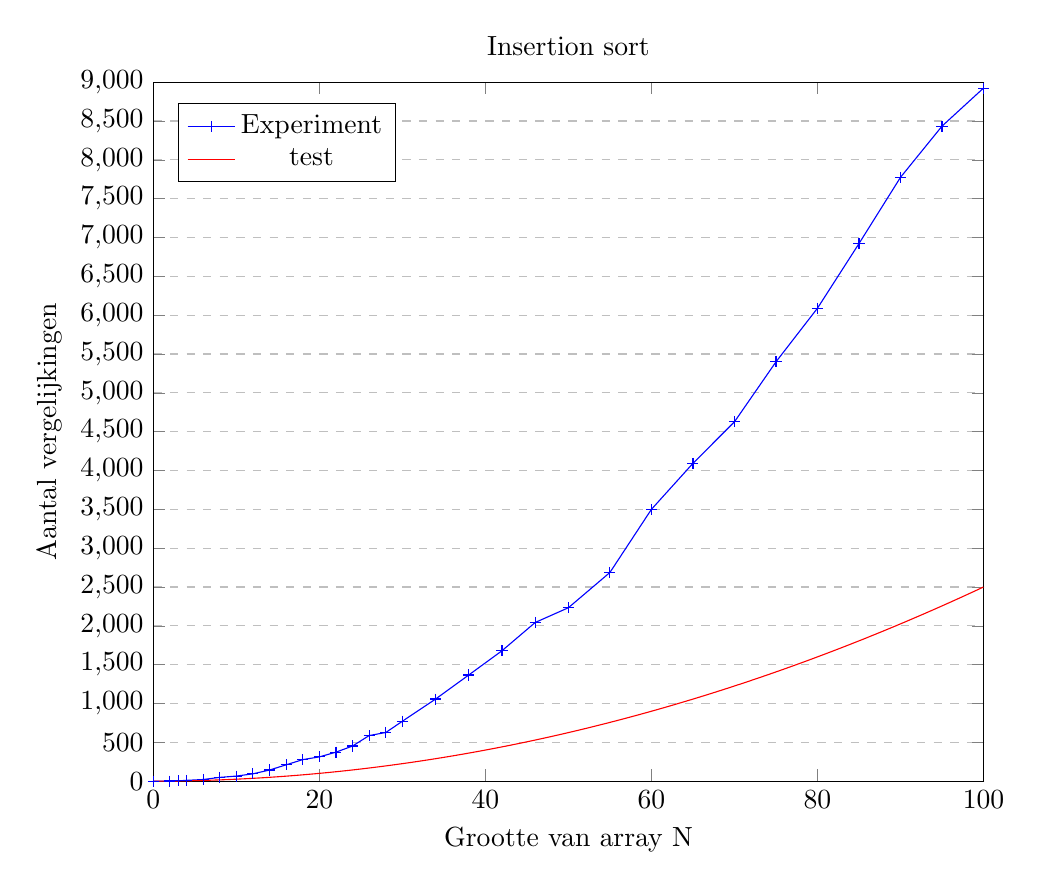
\begin{tikzpicture}
\begin{axis}[
    title={Insertion sort},
    xlabel={Grootte van array N},
    ylabel={Aantal vergelijkingen},
    xmin=0, xmax=100,
    ymin=0, ymax=9000,
    xtick={0,20,40,60,80,100},
    ytick={0,500,1000,1500,2000,2500,3000,3500,4000,4500,5000,5500,6000,6500,7000,7500,8000,8500,9000},
    legend pos=north west,
    ymajorgrids=true,
    grid style=dashed,
]
 
\addplot[
    color=blue,
    mark=+,
    ]
    coordinates {
    (0,0)(2,1)(3,4)(4,10)(6,21)(8,48)(10,65)(12,94)(14,143)(16,210)(18,277)(20,312)(22,373)(24,452)(26,587)(28,626)(30,771)(34,1057)(38,1367)(42,1679)(46,2043)(50,2233)(55,2687)(60,3500)(65,4092)(70,4627)(75,5399)(80,6090)(85,6922)(90,7775)(95,8434)(100,8924)
    };
    \legend{Experiment};

\addplot [
    domain= 0:100, 
    samples=100, 
    color=red,
    ]
    {(x^2)/4};
    \addlegendentry{test};
	
 
\end{axis}
\end{tikzpicture}

\subsubsection*{Quicksort}
\pgfplotstableread{
X Y
2 1
3 3
4 6
6 11
8 17
10 23
12 29
14 38
16 44
18 67
20 73
22 81
24 88
26 93	
28 107
30 127
34 141
38 156
42 166
46 259
50 274
55 306
60 325	
65 352
70 376
75 402
80 420
85 453
90 479
95 503
100 714
}\datatable
\begin{tikzpicture}
\begin{axis}[legend pos=outer north east]
\addplot [only marks, mark = *] table {\datatable};
\addplot [thick, red] table[
    y={create col/linear regression={y=Y}}
] % compute a linear regression from the input table
{\datatable};
\addlegendentry{$y(x)$}
\addlegendentry{%
$\pgfmathprintnumber{\pgfplotstableregressiona} \cdot x
\pgfmathprintnumber[print sign]{\pgfplotstableregressionb}$}
\end{axis}
\end{tikzpicture}

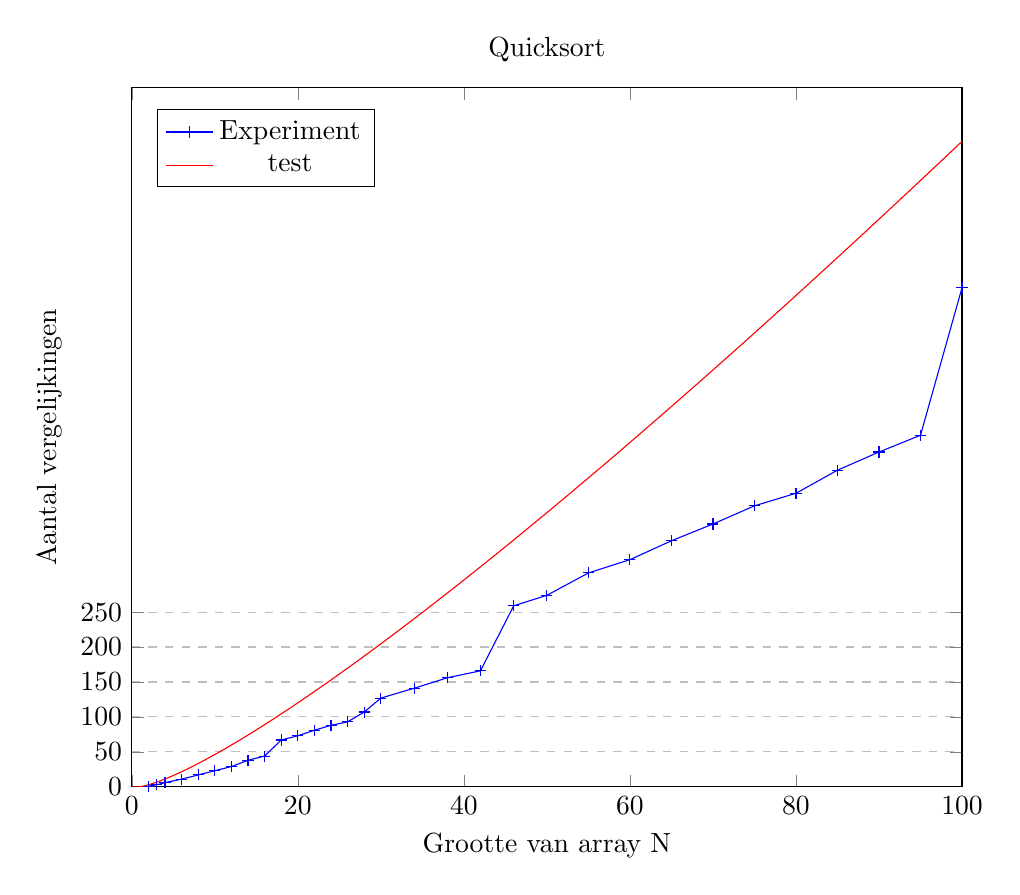
\begin{tikzpicture}
\begin{axis}[
    title={Quicksort},
    xlabel={Grootte van array N},
    ylabel={Aantal vergelijkingen},
    xmin=0, xmax=100,
    ymin=0, ymax=1000,
    xtick={0,20,40,60,80,100},
    ytick={0,50,100,150,200,250},
    legend pos=north west,
    ymajorgrids=true,
    grid style=dashed,
]
 
\addplot[
    color=blue,
    mark=+,
    ]
    coordinates {
	(2,1)(3,3)(4,6)(6,11)(8,17)(10,23)(12,29)(14,38)(16,44)(18,67)(20,73)(22,81)(24,88)(26,93)(28,107)(30,127)(34,141)(38,156)(42,166)(46,259)(50,274)(55,306)(60,325)(65,352)(70,376)(75,402)(80,420)(85,453)(90,479)(95,503)(100,714)
    };
    \legend{Experiment};

\addplot [
    domain= 0:100, 
    samples=100, 
    color=red,
    ]
    {1.39*x*(log2(x))};
    \addlegendentry{test};
	
 
\end{axis}
\end{tikzpicture}


\end{document}